\section{Robo-Sumo-Battle}\label{sec:RBS_design}


\subsection{Domænemodel for UC1 og UC2}

Med udgangspunkt i UC1 og UC2 er der blevet udarbejdet en domænemodel, der afspejler systemets individuelle delblokkes relationer og kommunikations metoder mellem hindanden. Domænemodellen vil være udgangspunkt til at designe systemets software. 

\begin{figure}
    \centering
    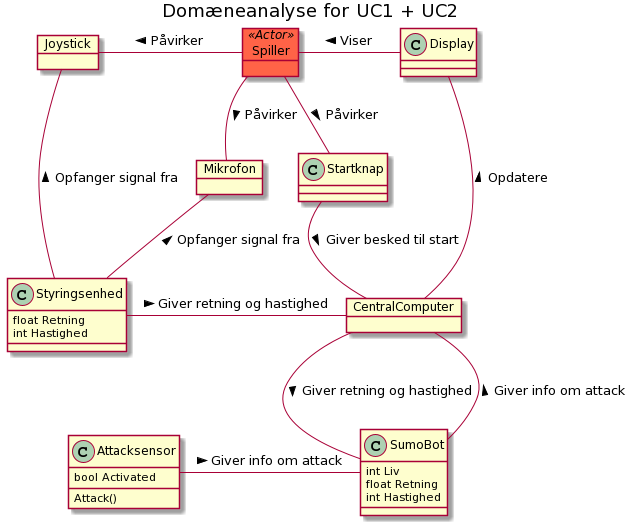
\includegraphics[width=\textwidth]{figs/Design/Central Computer/applikationsmodel/Domaenemodel.png}
    \caption{RSB Domænemodel}
    \label{fig:RSB_Domænemodel}
\end{figure}

\subsection{Communication Klasse}
Der er blevet udarbejdet et Communikation klassediagram, der vartager alle typer for digital kommunikation der skulle opstå mellem to eller flere delblokke. Dette klassediagram tagerudgangspunkt i delblokke fra domænemodellen \ref{Domænemodel} og samtlige IBD-diagrammer under strukturerings kapitlet. Communication klasse er blevet oprettet for at gøre systemet mere modtagelig for skallering. For at implementere nye led i systemet, f.eks. en version 2 af SumoBot, skal denne enhed blot være kompatible med Communication klassen. To (SumoBot og Central Computer) af de tre hoved elementer i systemet, (SumoBot, Central Computer og Styringsenhed) Vil benytte sig af "Communication" klassen.

***********klasse diagram ********

\subsubsection{\textbf{Communication}}
Communkation klassen er fællesledet mellem de forskellige kommunikation metoder der fremgår. Deri ligger der Send() og Revcieve() som vil blive overskrevet i forbindelse med hvilken arving et objekt oprettes ved.

*****UDSNIT FRA KLASSEDIAGRAM*******

\paragraph{Communication()}
\begin{functionDescription}
{Communication::Communication(??)}
{func:Communication}
{N/A}
{\textit{N/A}}{N/A}
\end{functionDescription}

\paragraph{Send()}
\begin{functionDescription}
{Communication::send(string msg)}
{func:send()}
{Funktionen oprettes som en virtuel funktion der vil overskrives af klasser der arver fra Communicaiton klassen F.eks TCPMaster,SPISlave mv..}
{\textit{Se attributter}}{N/A}
\end{functionDescription}

\paragraph{Receive()}
\begin{functionDescription}
{Communication::receive()}
{func:receive()}
{Funktionen oprettes som en virtuel funktion der vil overskrives af klasser der arver fra Communikaiton klassen F.eks TCPMaster,SPISlave mv.}
{\textit{Se attributter}}{N/A}
\end{functionDescription}


\paragraph{$\sim$ Communication()}
Destructor *****************sup


\subsubsection{Wifi}
Wifiklassen gør det muligt at oprette og nedlægge et hotspost, samt forbinde og afkoble til et. Klassen benytter sig af command line interface programmet Connman. REF TIL https://www.mankier.com/1/connmanctl\#Description


\paragraph{Attributter}

\begin{itemize}
    \item \textbf{string SSID} Navn på hotspottet  der oprettet, eller det som ønskes at forbindes til.
    \item \textbf{string passphrase} kodeord som giver adgang til et hotspot, evten ved oprettelse, eller forbindelse.
\end{itemize}

\paragraph{Metoder}

\begin{functionDescription}
{Wifin::Wifi()}
{func:Wifi}
{Sætter SSID og passphrase til default}
{\textit{N/A}}{N/A}
\end{functionDescription}

\begin{functionDescription}
{Wifi::createHotspot(string SSID, string passphrase)}
{func:createHotspot}
{Opretter et hotspot med et SSID (hotspotnavn) og et tilhørrende kodeord}
{{\begin{itemize}
    \item \textbf{string SSID} Navn på hotspot.
    \item \textbf{string passphrase} Kodeord til hotspot. 
\end{itemize}}}
{0 Hotspot blev oprettet. -1 SSID eller passphrase blev ikke sat korrekt. -2 Hotspot blev ikke aktiveret.}
\end{functionDescription}


\begin{functionDescription}
{Wifi::closeHotspot()}
{func:closeHotspot}
{Nedlægger det oprettet hotspot}
{N/A}
{0 hotspot blev deaktiveret. -1 Hotspot blev ikke deaktiveret korrekt}
\end{functionDescription}

\begin{functionDescription}
{Wifi::connectiToWifi(string SSID, string passphrase)}
{func:closeHotspot}
{Nedlægger det oprettet hotspot}
{{\begin{itemize}
    \item \textbf{string SSID} Navn på hotspot.
    \item \textbf{string passphrase} Kodeord til hotspot. 
\end{itemize}}}
{0 forbundet til hotspot. -1 Scanning for hotspots fejlede. -2 Ukendt AccesPoint, eller fejl i Connmanctl Connect. -3 Forkert kodet til hotspot. -4 SSID findes ikke.}
\end{functionDescription}

\begin{functionDescription}
{Wifi::disconnectiToWifi(string SSID)}
{func:disconnectToWifi}
{Nedlægger det oprettet forbindelse til hotspot}
{\textbf{string SSID} netværks navn der ønske at nedlægges forbindelse til}
{0 forbindelse nedlagt. -1 ukendt AccesPoint, ingen forbindelse nedlagt.-2 ukendt SSID.}
\end{functionDescription}

\begin{functionDescription}
{Wifi::$\sim$Wifi()}
{func: $\sim$Wifi}
{Nedlægger Hotspot eller forbindelse til hotspot. Udskriver på terminalen hvis fejl opstår}
{N/A}
{N/A}
\end{functionDescription}

\subsubsection{TCP}
\paragraph{Attributter}
\paragraph{TCP()}
\paragraph{Send()}
\paragraph{Receive()}
\paragraph{$\sim$TCP()}


\subsubsection{TCPClient}
\paragraph{Attributter}
\paragraph{TCPClient()}
\paragraph{ConnectToServer()}
\paragraph{Disconnect()}
\paragraph{$\sim$TCPClient()}


\subsubsection{TCPServer}
\paragraph{Attributter}
\paragraph{TCPServer()}
\paragraph{OpenServer()}
\paragraph{CloseServer()}
\paragraph{$\sim$TCPServer()}


\subsubsection{I2CMaster}
\paragraph{Attributter}
\paragraph{I2CMaster()}
\paragraph{Send()}
\paragraph{Receive()}
\paragraph{$\sim$I2CMaster()}


\subsubsection{I2CSlave}
\paragraph{Attributter}
\subsubsection{SPIMaster}
\paragraph{Attributter}
\paragraph{SPIMaster()}
\paragraph{Send()}
\paragraph{Receive()}
\paragraph{$\sim$SPIMaster()}


\subsubsection{SPISlave}
Da der i projektet ikke er behov for en SPI Slave på nuværende stadie, implementeres denne ikke. 

\subsubsection{SPIMaster}
Til kommunikation mellem styringsenhederne og centralcomputeren benyttes SPI, hvorfor vores kommunikationsklasse naturligvis også må have en SPI klasse. 

\textbf{Prerequisites:}
SPIMaster klassen benytter biblioteket wiringPi\textcolor{red}{INDSÆT REFERENCE}, som benyttes på tværs af projektet til kommunikation og GPIO manipulering fra userspace. 
\paragraph{Attributter}
SPIMaster klassen indeholder tre attributter:
\begin{itemize}
    \item \textbf{int fd:} En filedescriptor som peger på noden til SPI devicet. 
    \item \textbf{int bufferSize:} Størrelsen på bufferen i hvilken der sendes og modtages med (bemærk at disse er lige store for at overholde SPI protokollen). 
    \item \textbf{clkFrequency:} Clockfrekvensen med hvilken der overføres data. 
    \item \textbf{int channel:} SPIKanalen som benyttes
\end{itemize}
\paragraph{SPIMaster()}
\begin{functionDescription}
{SPIMaster::SPIMaster(int channel, int speed, int bufferSize)}
{func:SPIMaster}
{SPIMaster constructoren som sætter channel, speed og bufferSize}
{\textit{Se attributter}}
{N/A}
\end{functionDescription}
\paragraph{Send()}
\begin{functionDescription}
{int SPIMaster::send(string msg)}
{func:SPIMasterSend}
{Validerer at den modtagne tekststreng overholder wordsize (buffersize) og sender den herefter til den specifikke SPI kanal, med den korrekte hastighed, vha. en funktion fra wiringPi-biblioteket.}
{\begin{itemize}
    \item \textbf{string msg:} Meddelelsen som skal sendes afsted. Bemærk: Datatypen string er valgt for at SPIMaster klassen kan overwrite send funktionen i baseklassen, Communication.  
\end{itemize}}
{Returnerer -1 for en besked som ikke er afsendt pga forkert længde, og -2 for beskeder som ikke kunne afsendes af anden årsag og 0 for succesfuld afsendelse af besked}
\end{functionDescription}
\paragraph{sendChar()}
\begin{functionDescription}
{int SPIMaster::sendChar(unsigned char msg)}
{func:SPIMastersendChar}
{Denne funktion afsender blot ét enkelt byte}
{\begin{itemize}
    \item \textbf{unsigned char msg:} Den byte som ønskes afsendt
\end{itemize}}
{-1 for besked som ikke kunne afsendes. 0 for besked der succesfuld er blevet afsendt}
\end{functionDescription}
\paragraph{Receive()}
\begin{functionDescription}
{int SPIMaster::receive(char *buffer, int length)}
{func:SPIMaster_receive}
{Denne funktion modtager en besked via den tidligere angivne SPI-kanal og ved den angivne hastighed. Da SPI protokollen angiver at der skal sendes data for at modtage data, afsender funktionen tomt dummy-data}
{\begin{itemize}
    \item \textbf{char *buffer:} Pointer til den buffer hvori det modtagne data skal gemmes
    \item \textbf{int length:} Længden af det data som skal modtages. 
\end{itemize}}
{-1 for en besked som ikke kunne modtages og 0 for en succesfuld modtaget besked}
\end{functionDescription}
\paragraph{$\sim$SPIMaster()}
SPIMaster benytter en default destructor. 





\begin{functionDescription}
{Navn}
{func:label}
{Beskrivelse}
{Parametre}
{Returværdi}
\end{functionDescription}